\section{28. November 2018}
%! Hier gibts schon ein bisschen was hier: https://docs.google.com/document/d/1VvuRhqSy6umcpChijdMtuYw5qB0H7iJZGPXQbSMj6zA/edit
\question{Skizzieren Sie die wesentlichen Elemente der Born-Oppenheimer Näherung.}
\label{q:61}

Siehe \aqref{21}.

\question{Diskutieren Sie die sp-, sp$^2$-, sp$^3$-Hybridisierung in mehratomigen Molekülen.}
\label{q:62}

Hybridisierung bedeutet eine Mischung aus s- und p- Orbitalen,
hervorgerufen durch die Verformung der Elektronenhülle aufgrund
der Wechselwirkung zwischen den an der Bindung beteiligten Atomen.
Dabei gibt es die sp-, die sp$^2$- und die sp$^3$-Hybridisierung:

\begin{itemize}
    \item Eine sp-Hybridisierung führt zu zwei entgegengerichteten Bindungen und damit
          zu einem linearen Molekül, wenn keine anderen Bindungen vorhanden sind. Hier hybridisieren das 2s und ein 2p Orbital zu zwei sp-Orbitalen.
         
          \begin{figure}[H]
            \begin{minipage}[b]{0.5\linewidth} 
               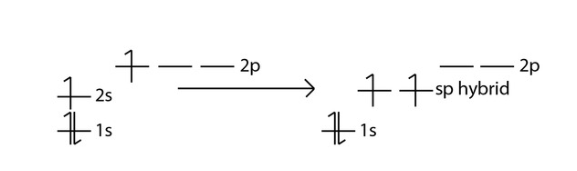
\includegraphics[width=0.8\linewidth]{resources/28-11-2018/sp11.PNG}
               \caption{sp-Hybridisierung, wobei die Energie sinkt}
            \end{minipage}
            \hspace{0.01\linewidth}
            \begin{minipage}[b]{0.5\linewidth} 
               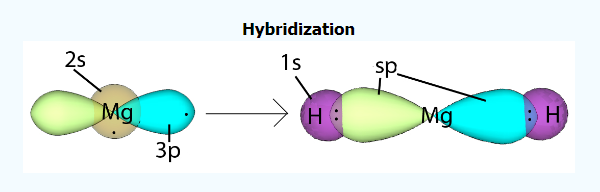
\includegraphics[width=0.8\linewidth]{resources/28-11-2018/sp12.PNG}
               \caption{sp-Hybridisierung am Beispiel von Magnesium }
            \end{minipage}
         \end{figure}

    \item Die sp$^2$-Hybridisierung führt zu drei gerichteten Bindungen, die in einer
          Ebene liegen. Hier bilden sich aus den 2s und zwei 2p-Orbitalen, drei sp-Orbitale.

          \begin{figure}[H]
            \begin{minipage}[b]{0.5\linewidth} 
               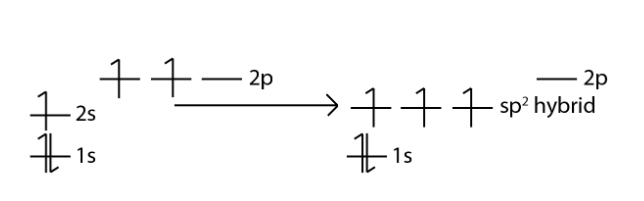
\includegraphics[width=0.8\linewidth]{resources/28-11-2018/sp21.PNG}
               \caption{sp$^2$-Hybridisierung, wobei die Energie sinkt}
            \end{minipage}
            \hspace{0.01\linewidth}
            \begin{minipage}[b]{0.5\linewidth} 
               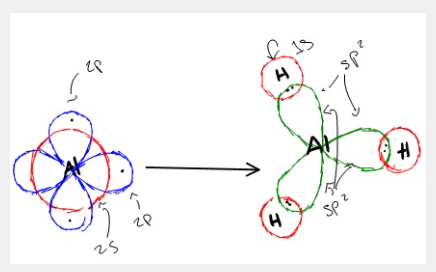
\includegraphics[width=0.8\linewidth]{resources/28-11-2018/sp22.PNG}
               \caption{sp$^2$-Hybridisierung am Beispiel von Aluminiumhydroxid}
            \end{minipage}
         \end{figure}

    \item Für die sp$^3$-Hybridisierung ergeben sich Atomorbitale mit Maxima, die in die vier Ecken eines Tetraeders zeigen.
          Hier bilden sich aus den 2s und drei 2p-Orbitalen, vier sp$^3$-Orbitale.

          \begin{figure}[H]
            \begin{minipage}[b]{0.5\linewidth} 
               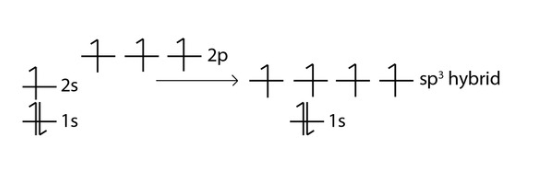
\includegraphics[width=0.8\linewidth]{resources/28-11-2018/sp31.PNG}
               \caption{sp$^3$-Hybridisierung, wobei die Energie sinkt}
            \end{minipage}
            \hspace{0.01\linewidth}
            \begin{minipage}[b]{0.5\linewidth} 
               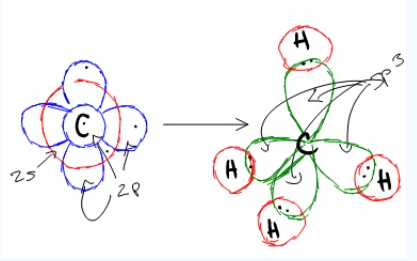
\includegraphics[width=0.8\linewidth]{resources/28-11-2018/sp32.PNG}
               \caption{sp$^3$-Hybridisierung am Beispiel von Methan}
            \end{minipage}
         \end{figure}

\end{itemize}

\question{Diskutieren Sie die Laue'sche Beugungsbedingung anhand der Ewald-Konstruktion im Rahmen der Bragg'schen Interpretation.}
\label{q:63}

Siehe \aqref{26}.

\question{Wodurch unterscheiden sich ein fcc-Gitter von einer hcp-Struktur?}
\label{q:64}

Siehe \aqref{46}.

\question{Diskutieren Sie die Gitterenergie der Ionenkristalle.}
\label{q:65}

Für die Berechnung der Gitterenergie in Ionenkristallen sind auch entferntere Nachbarn (nicht nur nächste) relevant. 
Die gesamte Bindungsenergie (Gitterenergie) $E_G$ ergibt sich zu: 
\[E_G = -\frac{N\cdot \alpha \cdot q^2}{4\pi\epsilon_0 R_0}(1-\nicefrac{\varrho}{R_0})\]
Sie hängt also von der Molekühlanzahl $N$, einem Abstoßungsparameter $\varrho$ und der Madelungkonstante $\alpha$ ab. $q$ ist wie gewohnt die Ladung und $R_0$ der Gleichgewichtsabstand zwischen Ionen. 

Zur Herleitung: (siehe auch Demtröder 3 S. 395-396)

Für \ch{Na+}--\ch{Cl-} folgt aus dem Experiment $R$(\ch{Na+}--\ch{Cl-}) = \SI{2.81}{\angstrom} und $E_{B,experimentell} = \SI{8.2}{\electronvolt}$.
Rechnet man über die Coulombenergie mit: 
\[E_{pot} = \frac{e^2}{4\pi\epsilon_0 R} = \SI{5.1}{eV}\]
erhält man einen wesentlich kleineren Wert $\rightarrow$ weitere nächste Nachbarn müssen berücksichtigt werden.
Nun kann man das Potential zwischen zwei Ionen beschreiben als: 
\[E_{pot}^{(i,j)} = C \cdot e^{-r_{ij}/\varrho}\pm \frac{q^2}{4\pi\epsilon_0 r_{ij}} \rightarrow E_{pot}^{(i)} = \sum_{i \ne j} \left( C \cdot e^{-r_{ij}/\varrho}\pm \frac{q_i q_j}{4\pi\epsilon_0 r_{ij}} \right)\]
wobei $C$ eine Konstante ist, $r_{ij}$ der Abstand zwischen den Ionen $i$ und $j$ und $\varrho$ ein Abstoßungsparameter welcher den Abstand an der Stelle wo die Abstoßungsenergie auf 1/e abgefallen ist beschreibt. Die Exponentialfunktion beschreibt den abstoßenden Teil des Potentials bei Überlappung der innereren Elektronenschalen. \\
Nun werden für die Exponentialfunktion nur die nächsten Nachbarn betrachtet: 
\[E_{pot}^{(i)} = Z_{nN} \cdot C \cdot e^{-R_{nN}/\varrho}+\frac{q^2}{4\pi\epsilon_0} \sum_j\frac{\pm 1}{p_{ij}R_{nN}} = Z_{nN} \cdot C \cdot e^{-R_{nN}/\varrho}+\frac{\alpha q^2}{4\pi\epsilon_0 R_{nN}}\]
Hier ist $r_{ij} = p_{ij} \cdot R_{nN}$ wobei $R_{nN}$ der Abstand zu den nächsten Nachbarn ist. Letztlich wurde die \textbf{Madelungkonstante}: 
\[\alpha = \sum_j \frac{\mp 1}{p_{ij}}\]
eingesetzt. Letztendlich folgt also für $N$ Moleküle:
\[E_G = N \cdot E_{pot}^{(i)}\]
was bei $R_0$ sich nicht ändern darf: sprich $\left(\frac{d E_{pot}^{(i)}}{d R}\right)_{R_0} = 0$ ableiten und umformen ergibt obige Gleichung. 

Der Hauptanteil der Bindungsenergie von Ionenkristallen ist die Coulomb-Energie. 

\question{Vergleichen Sie die Einstein- und Debye-Modelle der spezifischen Wärme. Welche Annahmen sind in beiden Modellen zu einfach?}
\label{q:66}

Siehe \aqref{57}.

\question{Diskutieren Sie das Auftreten einer Energiebandlücke mit Hilfe des Modells der fast freien Elektronen.}
\label{q:67}

Siehe \aqref{5}.

\question{Wodurch unterscheidet sich die Dispersionsrelation der Phononen eines primitiven kubischen Gitters von jenem eines CsCl-Gitters.}
\label{q:68}

Siehe \aqref{49}.

\question{Erklären Sie die chemische Bindung von \ch{O2} ($Z=8$).}
\label{q:69}

\[\ch{O2} : (1\sigma_g)^2 ~ (1\sigma_u^*)^2 ~ (2\sigma_g)^2 ~ (2\sigma_u^*)^2 ~ (3\sigma_g)^2 ~ (1\pi_g)^4 ~ (1\pi_u^*)^2\]

Da beiden Sauerstoffatomen je zwei Elektronen auf Edelgaskonfiguration fehlen (sechs Valenzelektronen), kommt es zu einer Doppelbindung.

\setcapindent{0pt}
\begin{figure}[H]
   \centering
   \begin{minipage}[t]{0.475\linewidth}
      \centering
      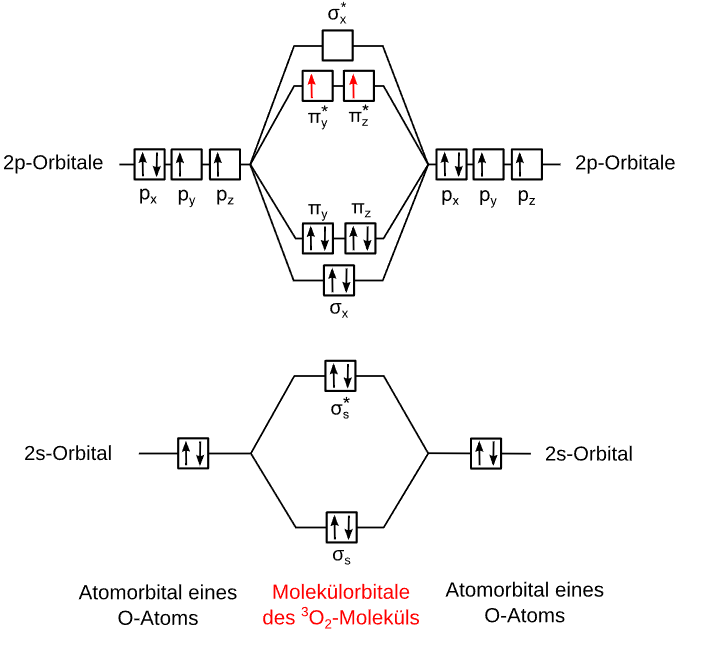
\includegraphics[width=\linewidth]{resources/28-11-2018/O2.PNG}
      \caption{Elektronenkonfiguration von \ch{O2}}
      \label{fig:Elektronenkonfiguration_O2}
   \end{minipage}%
   \hspace*{\fill}
   \begin{minipage}[t]{0.475\linewidth}
      \centering
      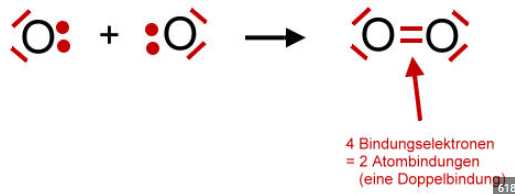
\includegraphics[width=\linewidth]{resources/28-11-2018/o2_bindung.PNG}
      \caption{Chemische Bindung zweier Sauerstoffatome}
      \label{fig:chemische_Bindung_O2}
   \end{minipage}
\end{figure}
\setcaphanging

\newpage